% \begin{frame}{Proposta}
%     Desenvolver um framework baseado em arquiteturas paralelas para escalonamento de tarefas em Edge-Cloud Continuum (ECC).
%     \vspace{1em}
%     \begin{enumerate}
%         \item Trabalhos relacionados.
%         \item Algoritmos.
%         \begin{itemize}
%             \item Algoritmos Determinísticos.
%             \item Arquiteturas Paralelas.
%         \end{itemize}
%         \item Cenário de execução.
%         \item Técnicas e ferramentas.
%         \item Cenário de teste.
%     \end{enumerate}
% \end{frame}

\begin{frame}{Algoritmos Determinísticos}
    Algoritmos Determinísticos:

    \begin{itemize}
        \item Resultados consistentes para determinada entrada.
        \item Previsíveis.
        \item Garantia de solução ótima.
        \item Características essenciais para garantir confiabilidade no sistema.
    \end{itemize}
\end{frame}

\begin{frame}{Arquiteturas Paralelas}
    Arquiteturas Paralelas:

    \begin{itemize}
        \item \textit{SIMD} e \textit{MIMD}.
        \item Otimizar a execução de operações em grandes volumes de dados.
        \item Alto desempenho.
    \end{itemize}
\end{frame}

\begin{frame}{Trabalhos Relacionados}
    \begin{figure}
        \centering
        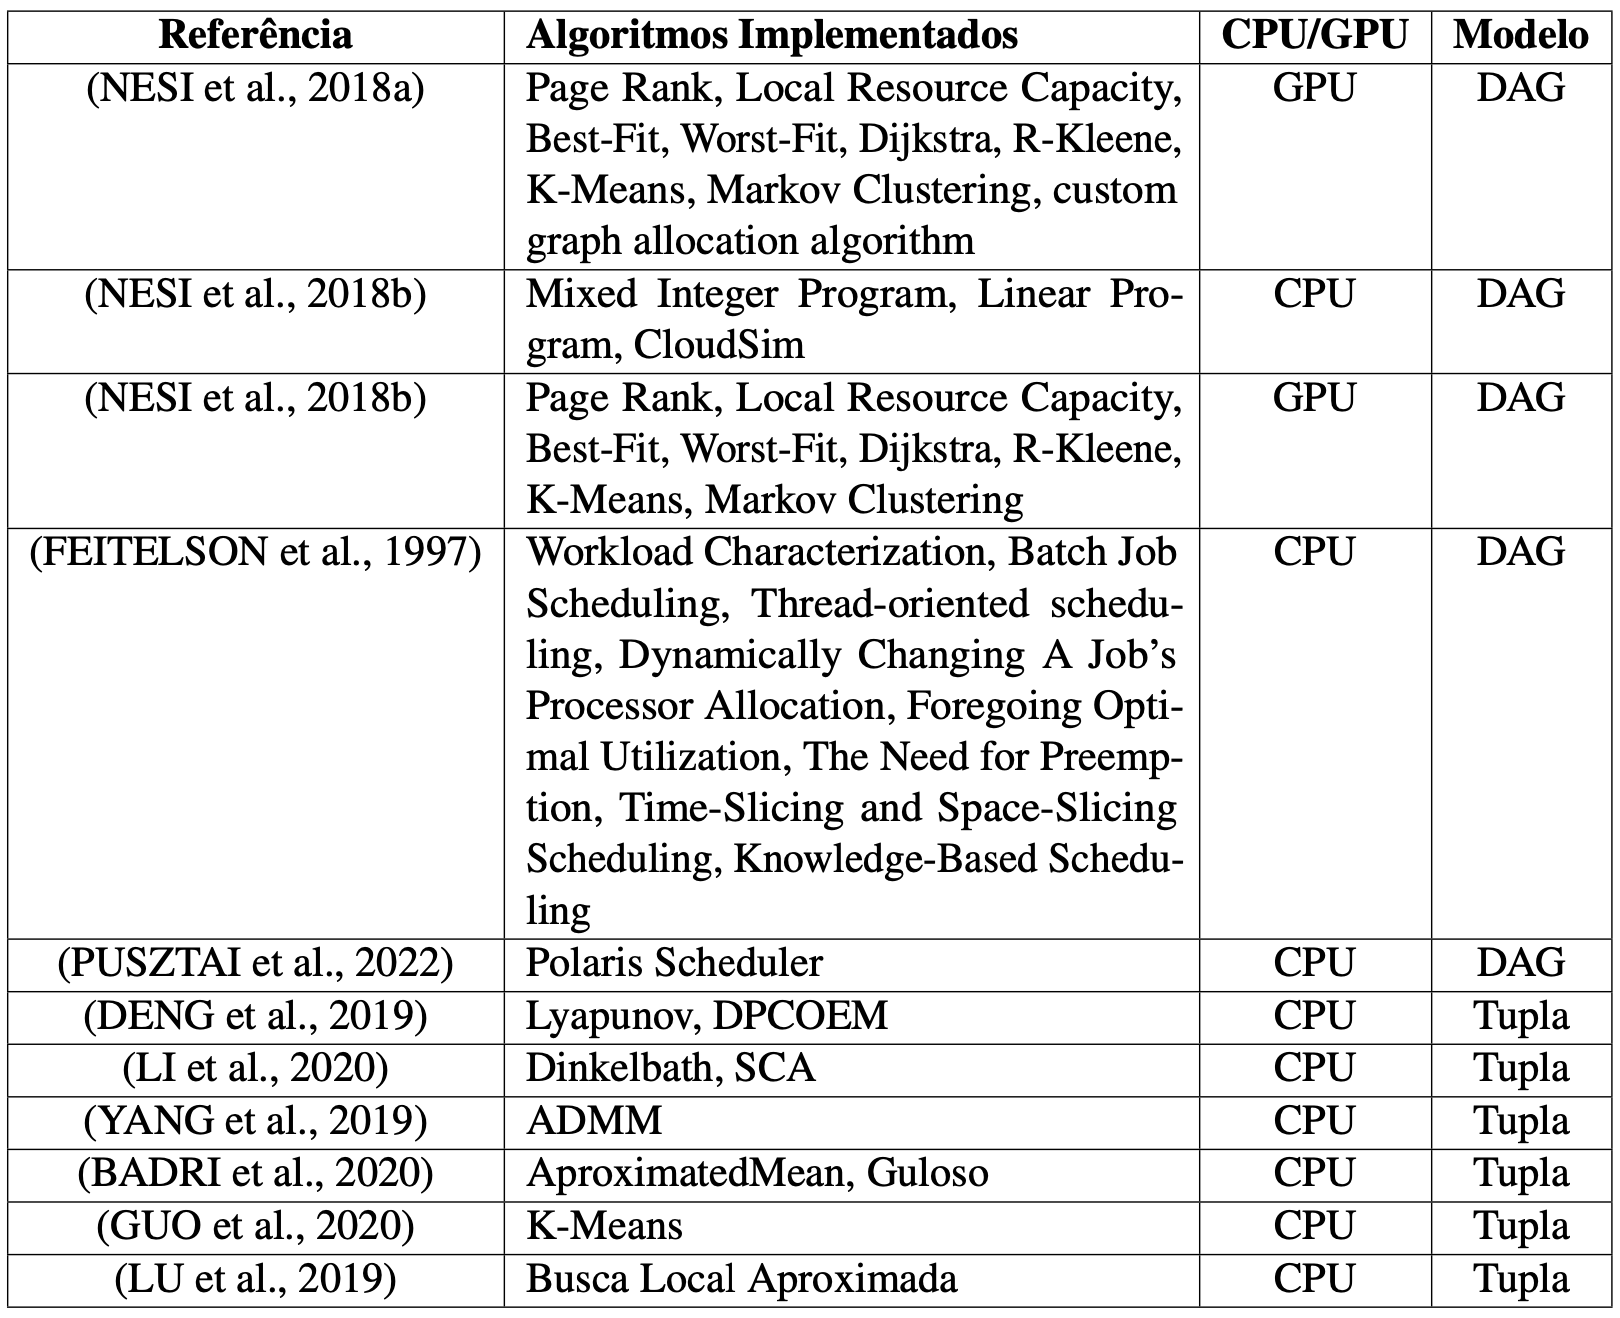
\includegraphics[width=0.9\textwidth]{Figuras/trabalhos-relacionados.png}
    \end{figure}
\end{frame}

\begin{frame}{Algoritmos}
    \begin{table}[ht]
        \centering
        \scriptsize
        \begin{tabular}{|c|c|c|c|}
            \hline
            \textbf{Algoritmo} & \textbf{Categoria} & \textbf{Complexidade} & \textbf{CPU/GPU} \\
            \hline
            Prefix Sum & DP & $O(n)$ & GPU \\
            \hline
            Busca Binária & Busca & $O(\log n)$ & CPU \\
            \hline
            Merge Sort & Ordenação & $O(n \log n)$ & CPU \\
            \hline
            Topological Sort & Ordenação & $O(V + E)$ & CPU \\
            \hline
            Radix Sort & Ordenação & $O(nw)$ & GPU \\
            \hline
            K-means & Agrupamento & $O(nkdi)$ & GPU \\
            \hline
            DBSCAN & Agrupamento & $O(n^2)$ & GPU \\
            \hline
            Hierarchical Clustering & Agrupamento & $O(n^3)$ & CPU \\
            \hline
            Markov Clustering & Agrupamento & $O(n^3)$ & GPU \\
            \hline
            PageRank & Ranqueamento & $O(n + m)$ & GPU \\
            \hline
            Dijkstra & Menor Caminho & $O(E + V \log V)$ & CPU \\
            \hline
            Floyd-Warshall & Menor Caminho & $O(n^3)$ & CPU \\
            \hline
            A* & Menor Caminho & $O(E \log V)$ & CPU \\
            \hline
            Kruskal & MST & $O(E \log E)$ & CPU \\
            \hline
            Prim & MST & $O(E + V \log V)$ & CPU \\
            \hline
            Edmonds-Karp & Fluxo & $O(VE^2)$ & CPU \\
            \hline
            Min-Cost Max-Flow & Fluxo & $O(V^2E^2)$ & CPU \\
            \hline
            Dinic & Fluxo & $O(V^2E)$ & CPU \\
            \hline
            Gaussian Elimination & Otimização & $O(n^3)$ & GPU \\
            \hline
            Hungarian & Otimização & $O(n^3)$ & CPU \\
            \hline
        \end{tabular}
        \caption{Algoritmos candidatos a serem implementados no \textit{framework}.}
        \label{table:algorithms}
    \end{table}
\end{frame}

% talvez remover esse slide
\begin{frame}{Cenário de execução}
    \begin{figure}
        \centering
        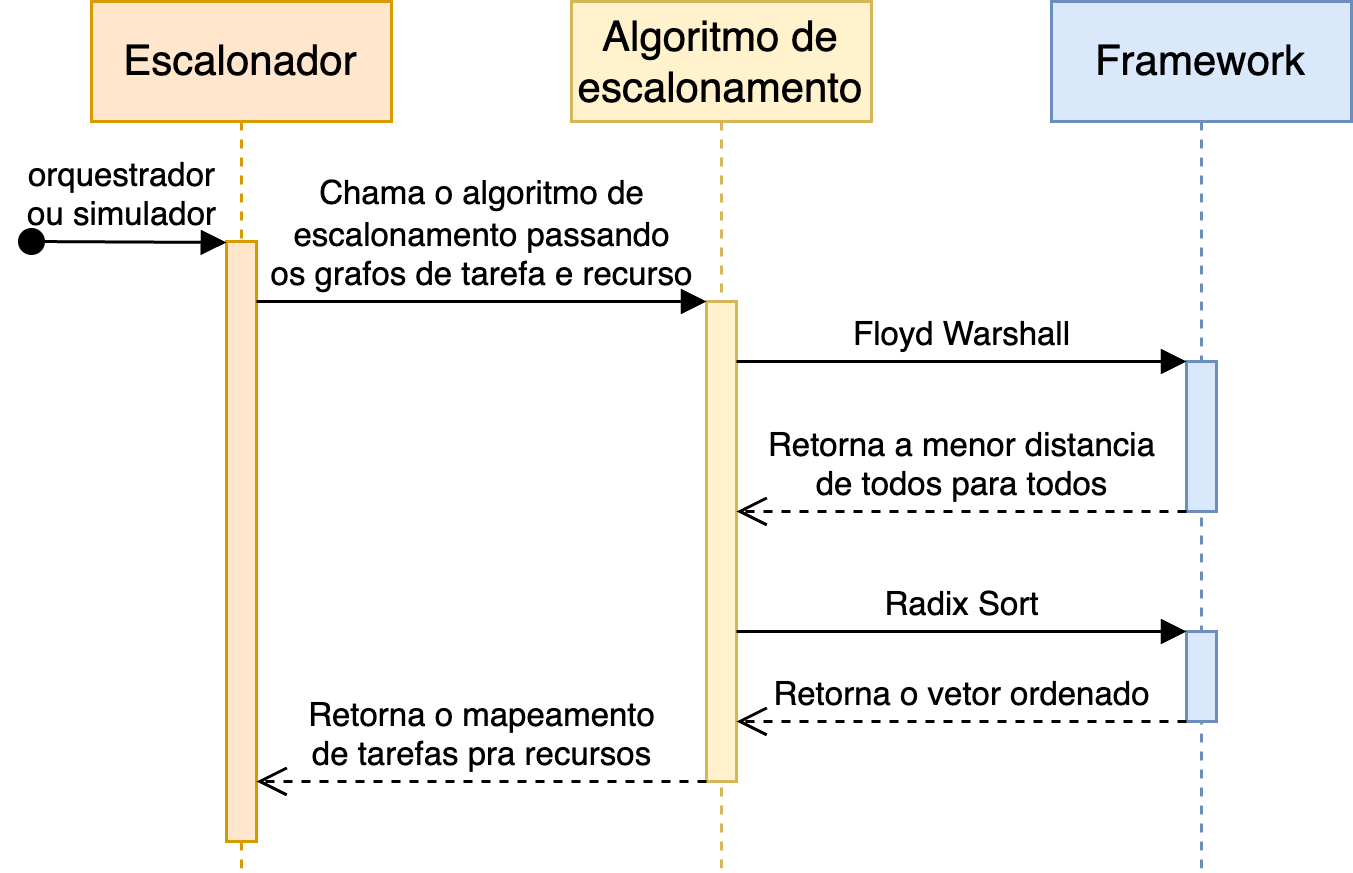
\includegraphics[width=\textwidth]{Figuras/framework-usage-2.png}
    \end{figure}
\end{frame}

\begin{frame}{Código Exemplo}
    \begin{figure}
        \centering
        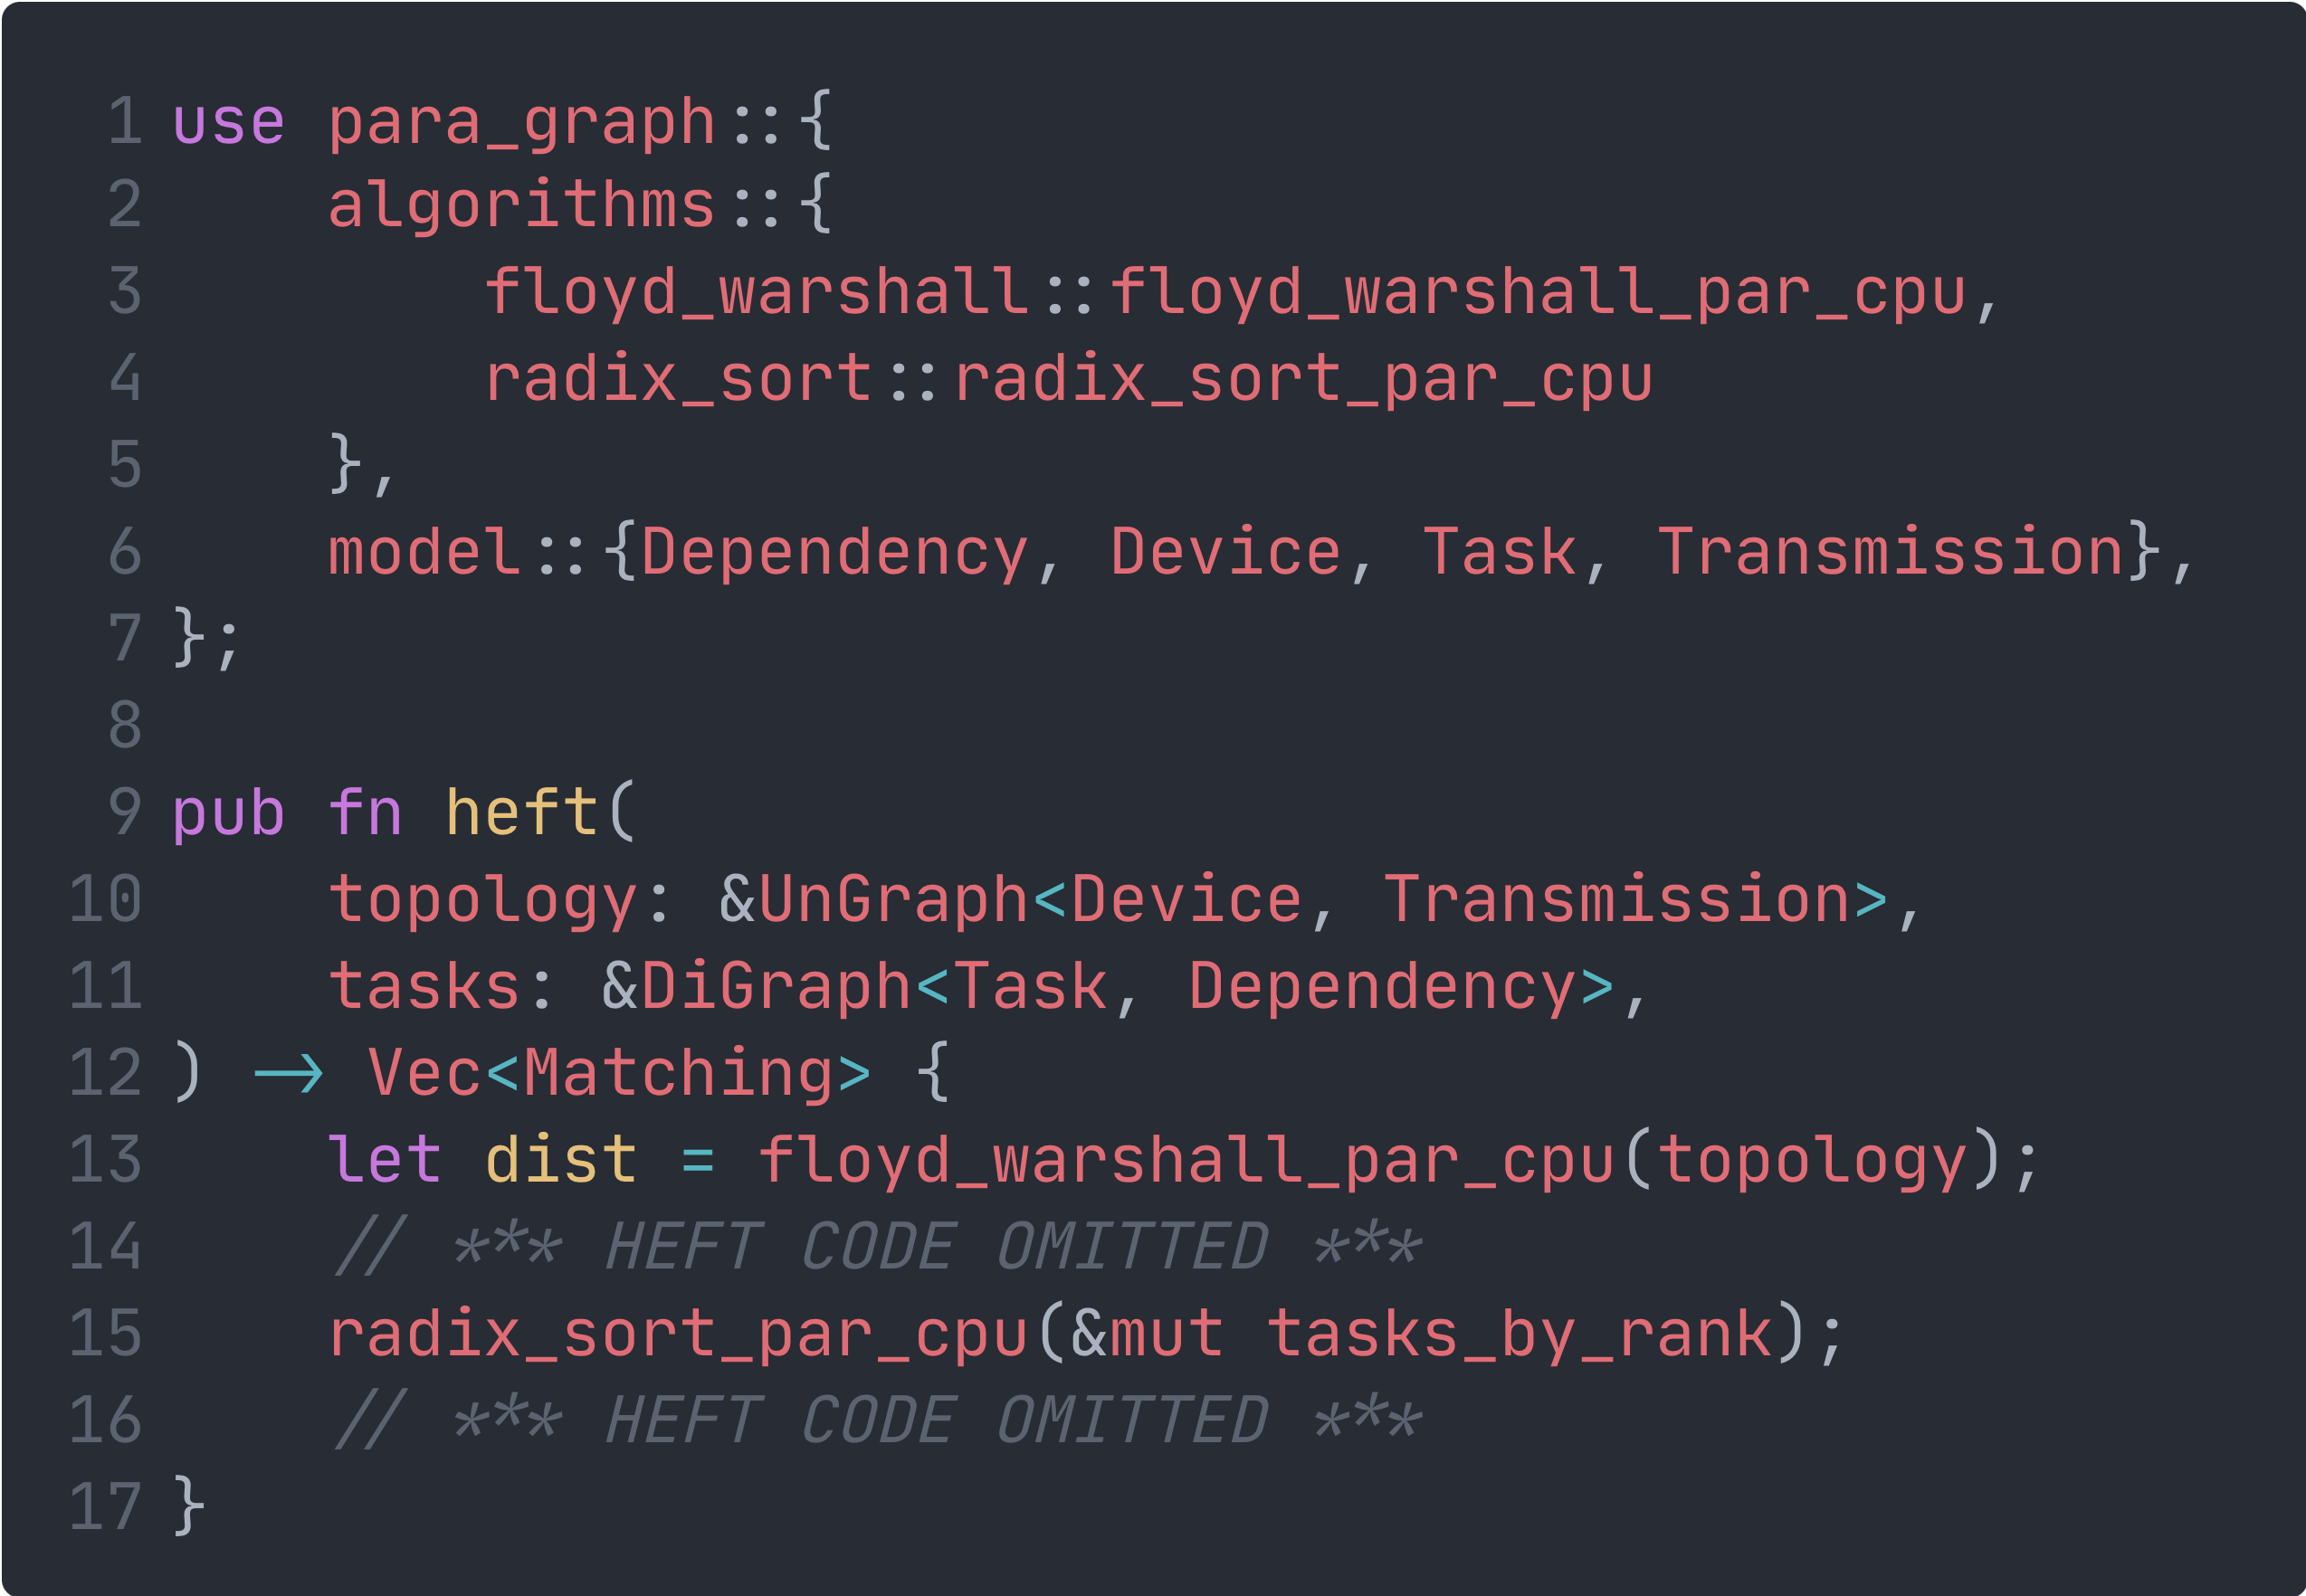
\includegraphics[width=\textwidth]{Figuras/code-2.png}
    \end{figure}
\end{frame}

\begin{frame}{Técnicas e Ferramentas}
    \begin{columns}
    \begin{column}{0.9\textwidth}
    Rust:
    \begin{itemize}
        \item[--] Linguagem moderna.
        \item[--] Segurança de memória.
        \item[--] Alto desempenho. 
        \item[--] \textit{Petgraph}.
        \item[--] \textit{Rayon}.
        \item[--] \textit{Fearless Concurrency}.
    \end{itemize}
    \end{column}

    \begin{column}{0.1\textwidth}
        \begin{figure}
            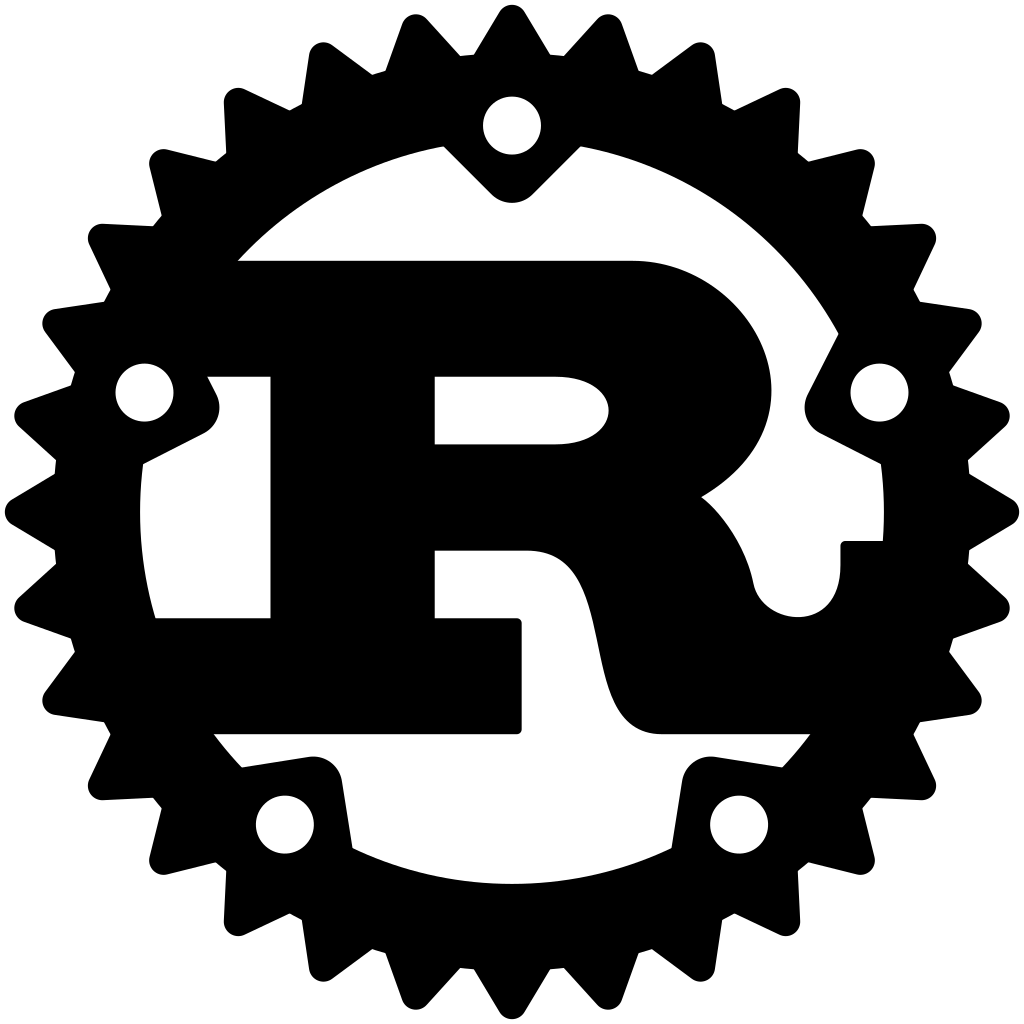
\includegraphics[width=\textwidth]{Figuras/Rust Logo.svg.png}
        \end{figure}
    \end{column}
    \end{columns}
\end{frame}

% \begin{frame}{Fearless Concurrency}
%     \begin{figure}
%         \centering
%         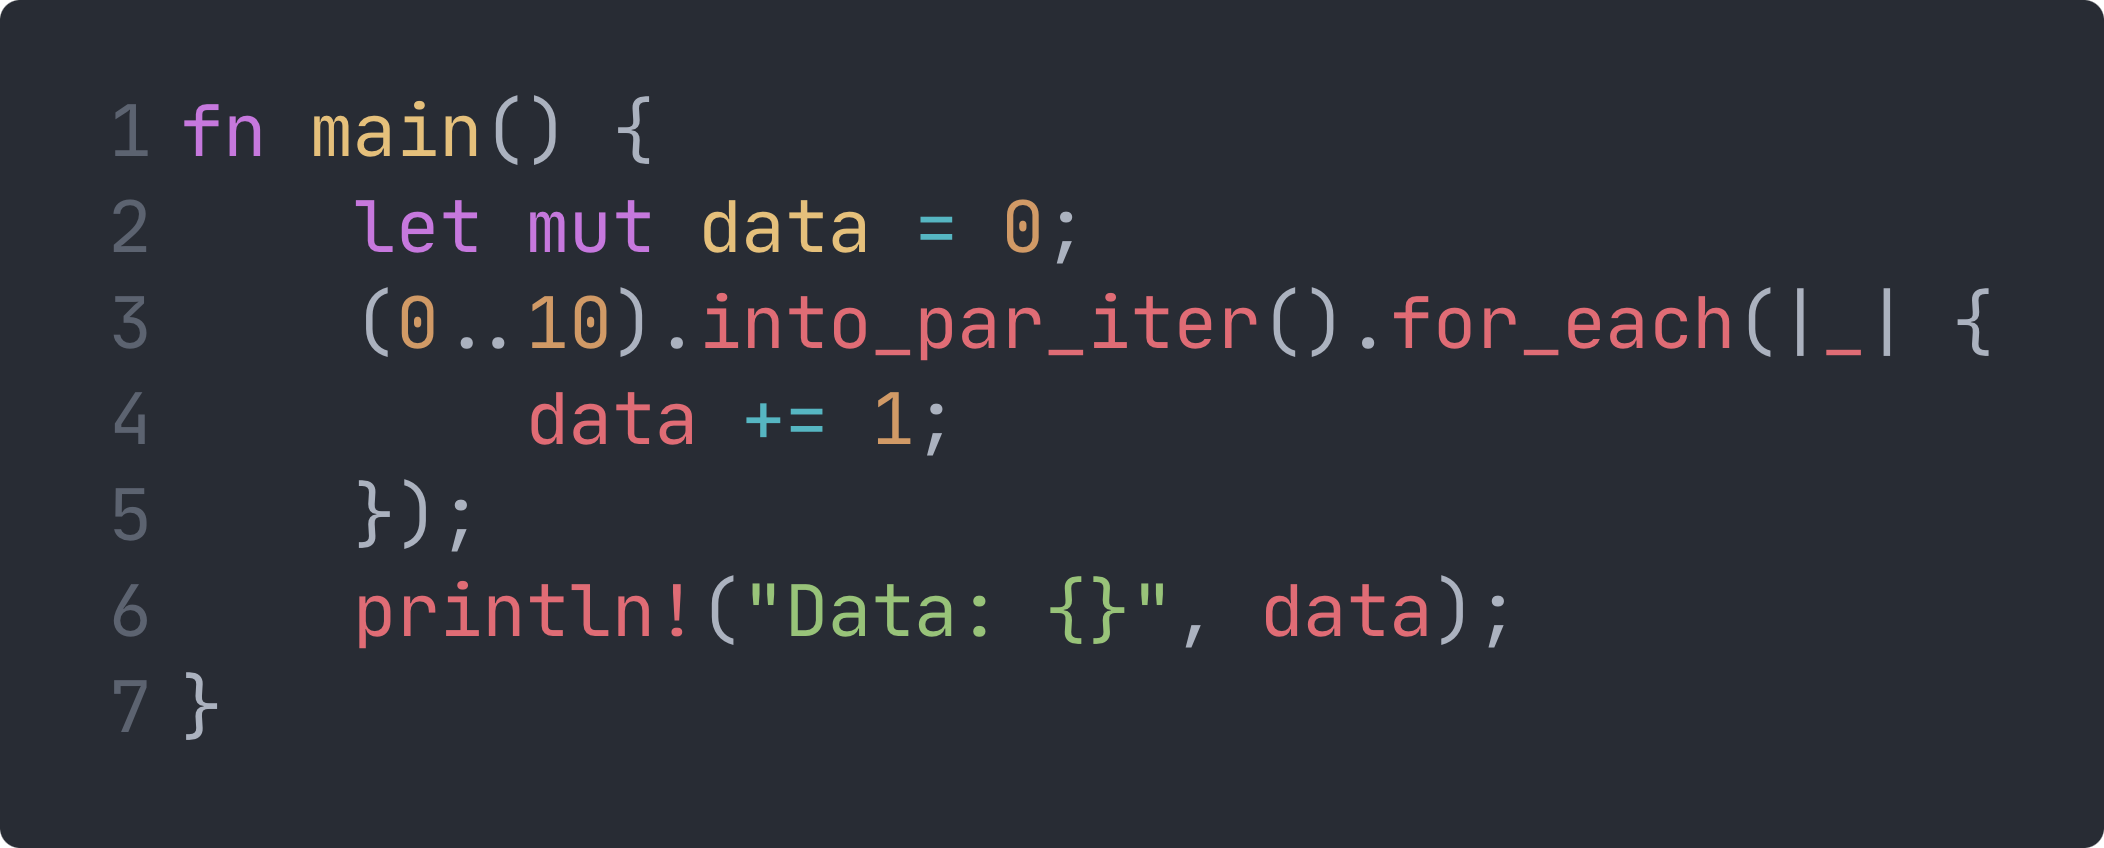
\includegraphics[width=\textwidth]{Figuras/fearlessconcurrency.png}
%     \end{figure}
% \end{frame}

\begin{frame}{Técnicas e Ferramentas}
    \begin{columns}
    \begin{column}{0.9\textwidth}
    C++:
    \begin{itemize}
        \item[--] Excelente suporte a \textit{GPUs}.
        \item[--] \textit{OpenAcc}.
        \item[--] Comunicação por meio de \textit{Foreign Function Interface}.
    \end{itemize}
    \end{column}

    \begin{column}{0.1\textwidth}
        \begin{figure}
            
\includegraphics[width=\textwidth]{Figuras/C++ Logo.png}
        \end{figure}
    \end{column}
    \end{columns}
\end{frame}

\begin{frame}{Código Exemplo}
    \begin{figure}
        \centering
        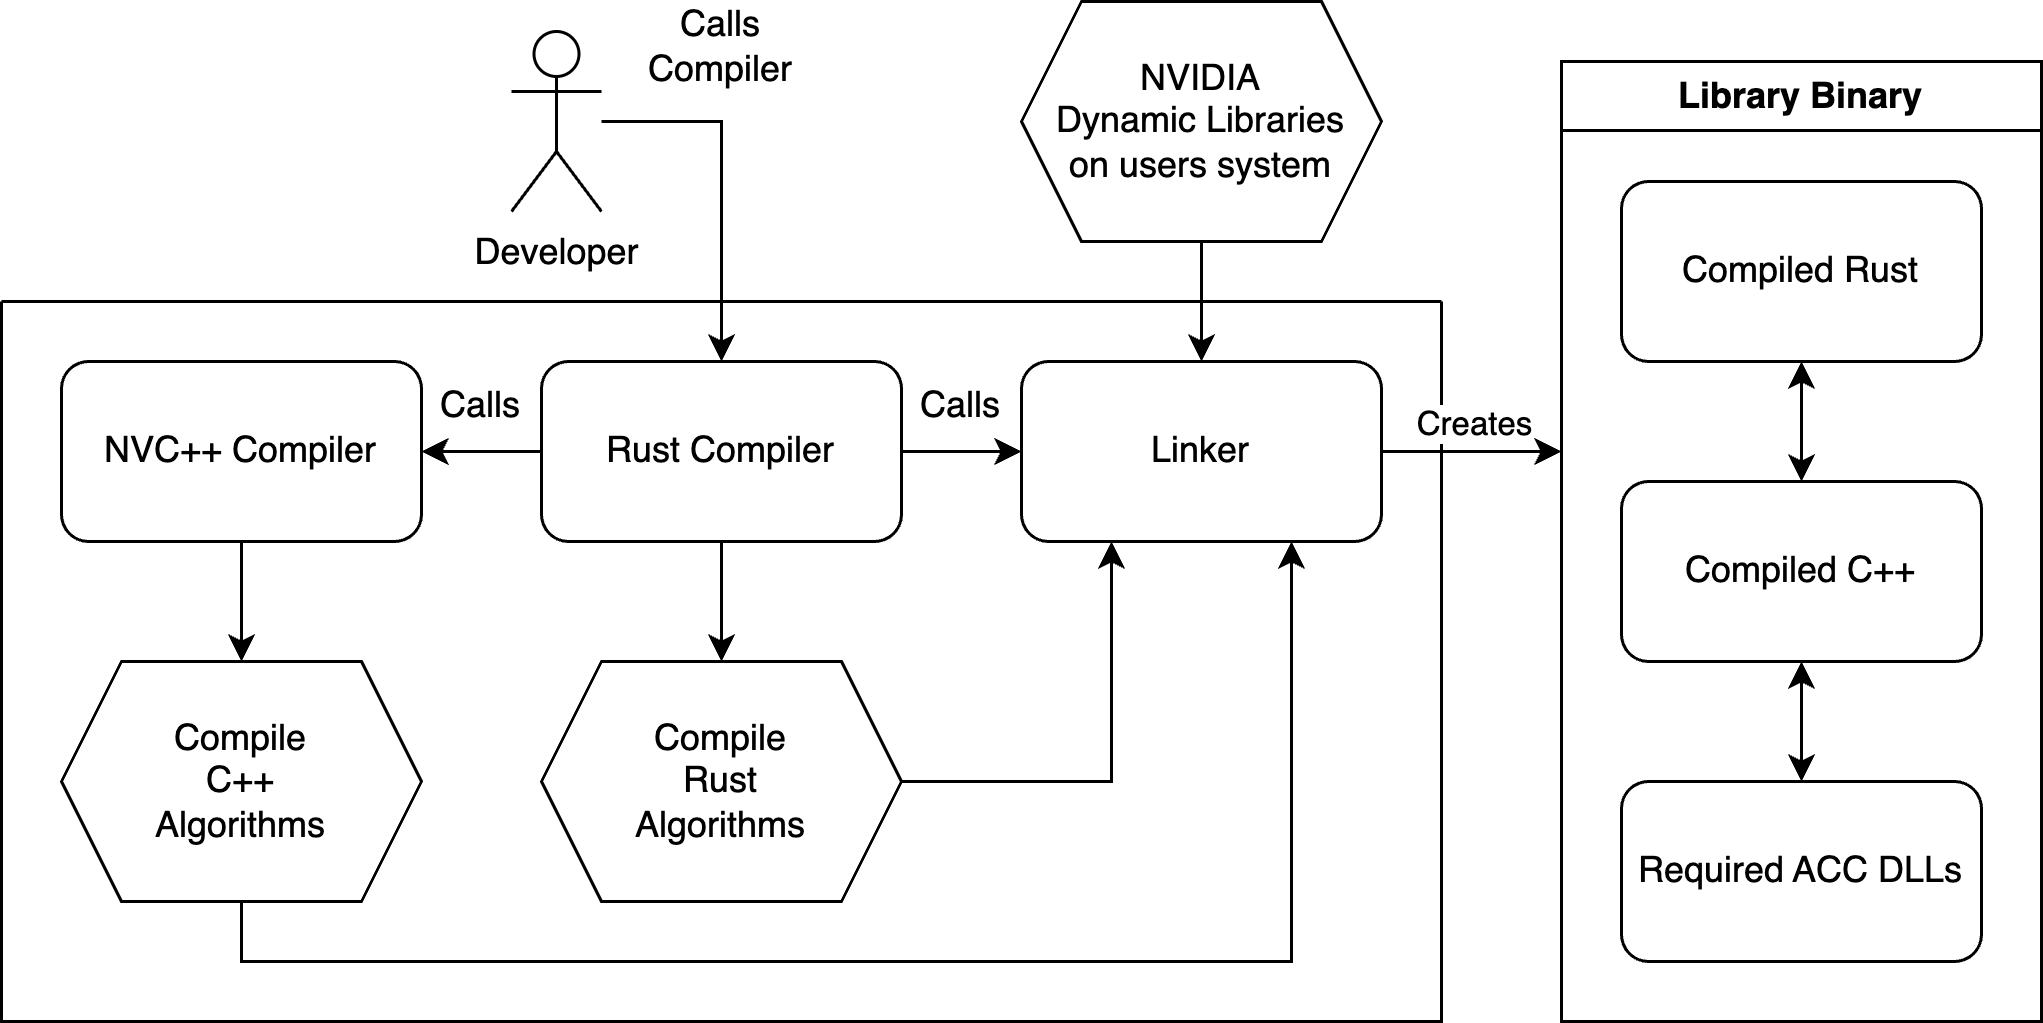
\includegraphics[width=\textwidth]{Figuras/TCC Compilacao.png}
    \end{figure}
\end{frame}

\begin{frame}{Algoritmos}
    \begin{enumerate}
        \item Prefix Sum.
        \item Busca Binária.
        \item Radix Sort.
        \item Floyd Warshall.
        \item Gauss Elimination.
    \end{enumerate}
\end{frame}

\begin{frame}{Prefix Sum}
    \begin{figure}
        \centering
        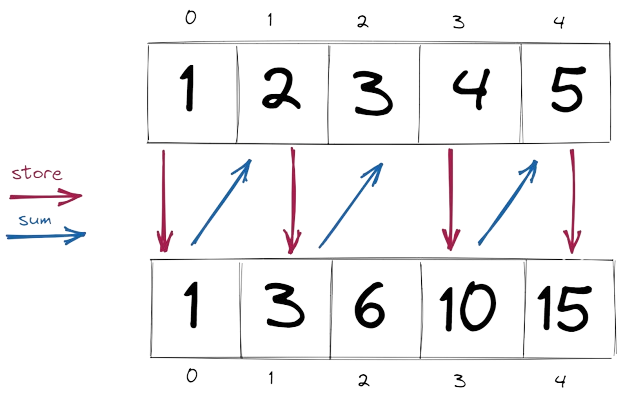
\includegraphics[width=\textwidth]{Figuras/PrefixSum.png}
    \end{figure}
\end{frame}

\begin{frame}{Prefix Sum}
    Se resume em gerar uma nova lista a partir de uma lista de entrada, na qual um elemento na posição $i$ é a soma dos elementos das posições $0$ até $i$ da lista original.
    \vspace{1em}
    \begin{itemize}
        \item \textbf{Serial:} Algoritmo Trivial $O(n)$.
        \item \textbf{CPU:} Algoritmo de dois passos $O(n)$.
        \item \textbf{GPU:} Algoritmo de \textit{Blelloch} $O(n \log n)$.
    \end{itemize}
\end{frame}

\begin{frame}{Prefix Sum Paralelo}
    \begin{figure}
        \centering
        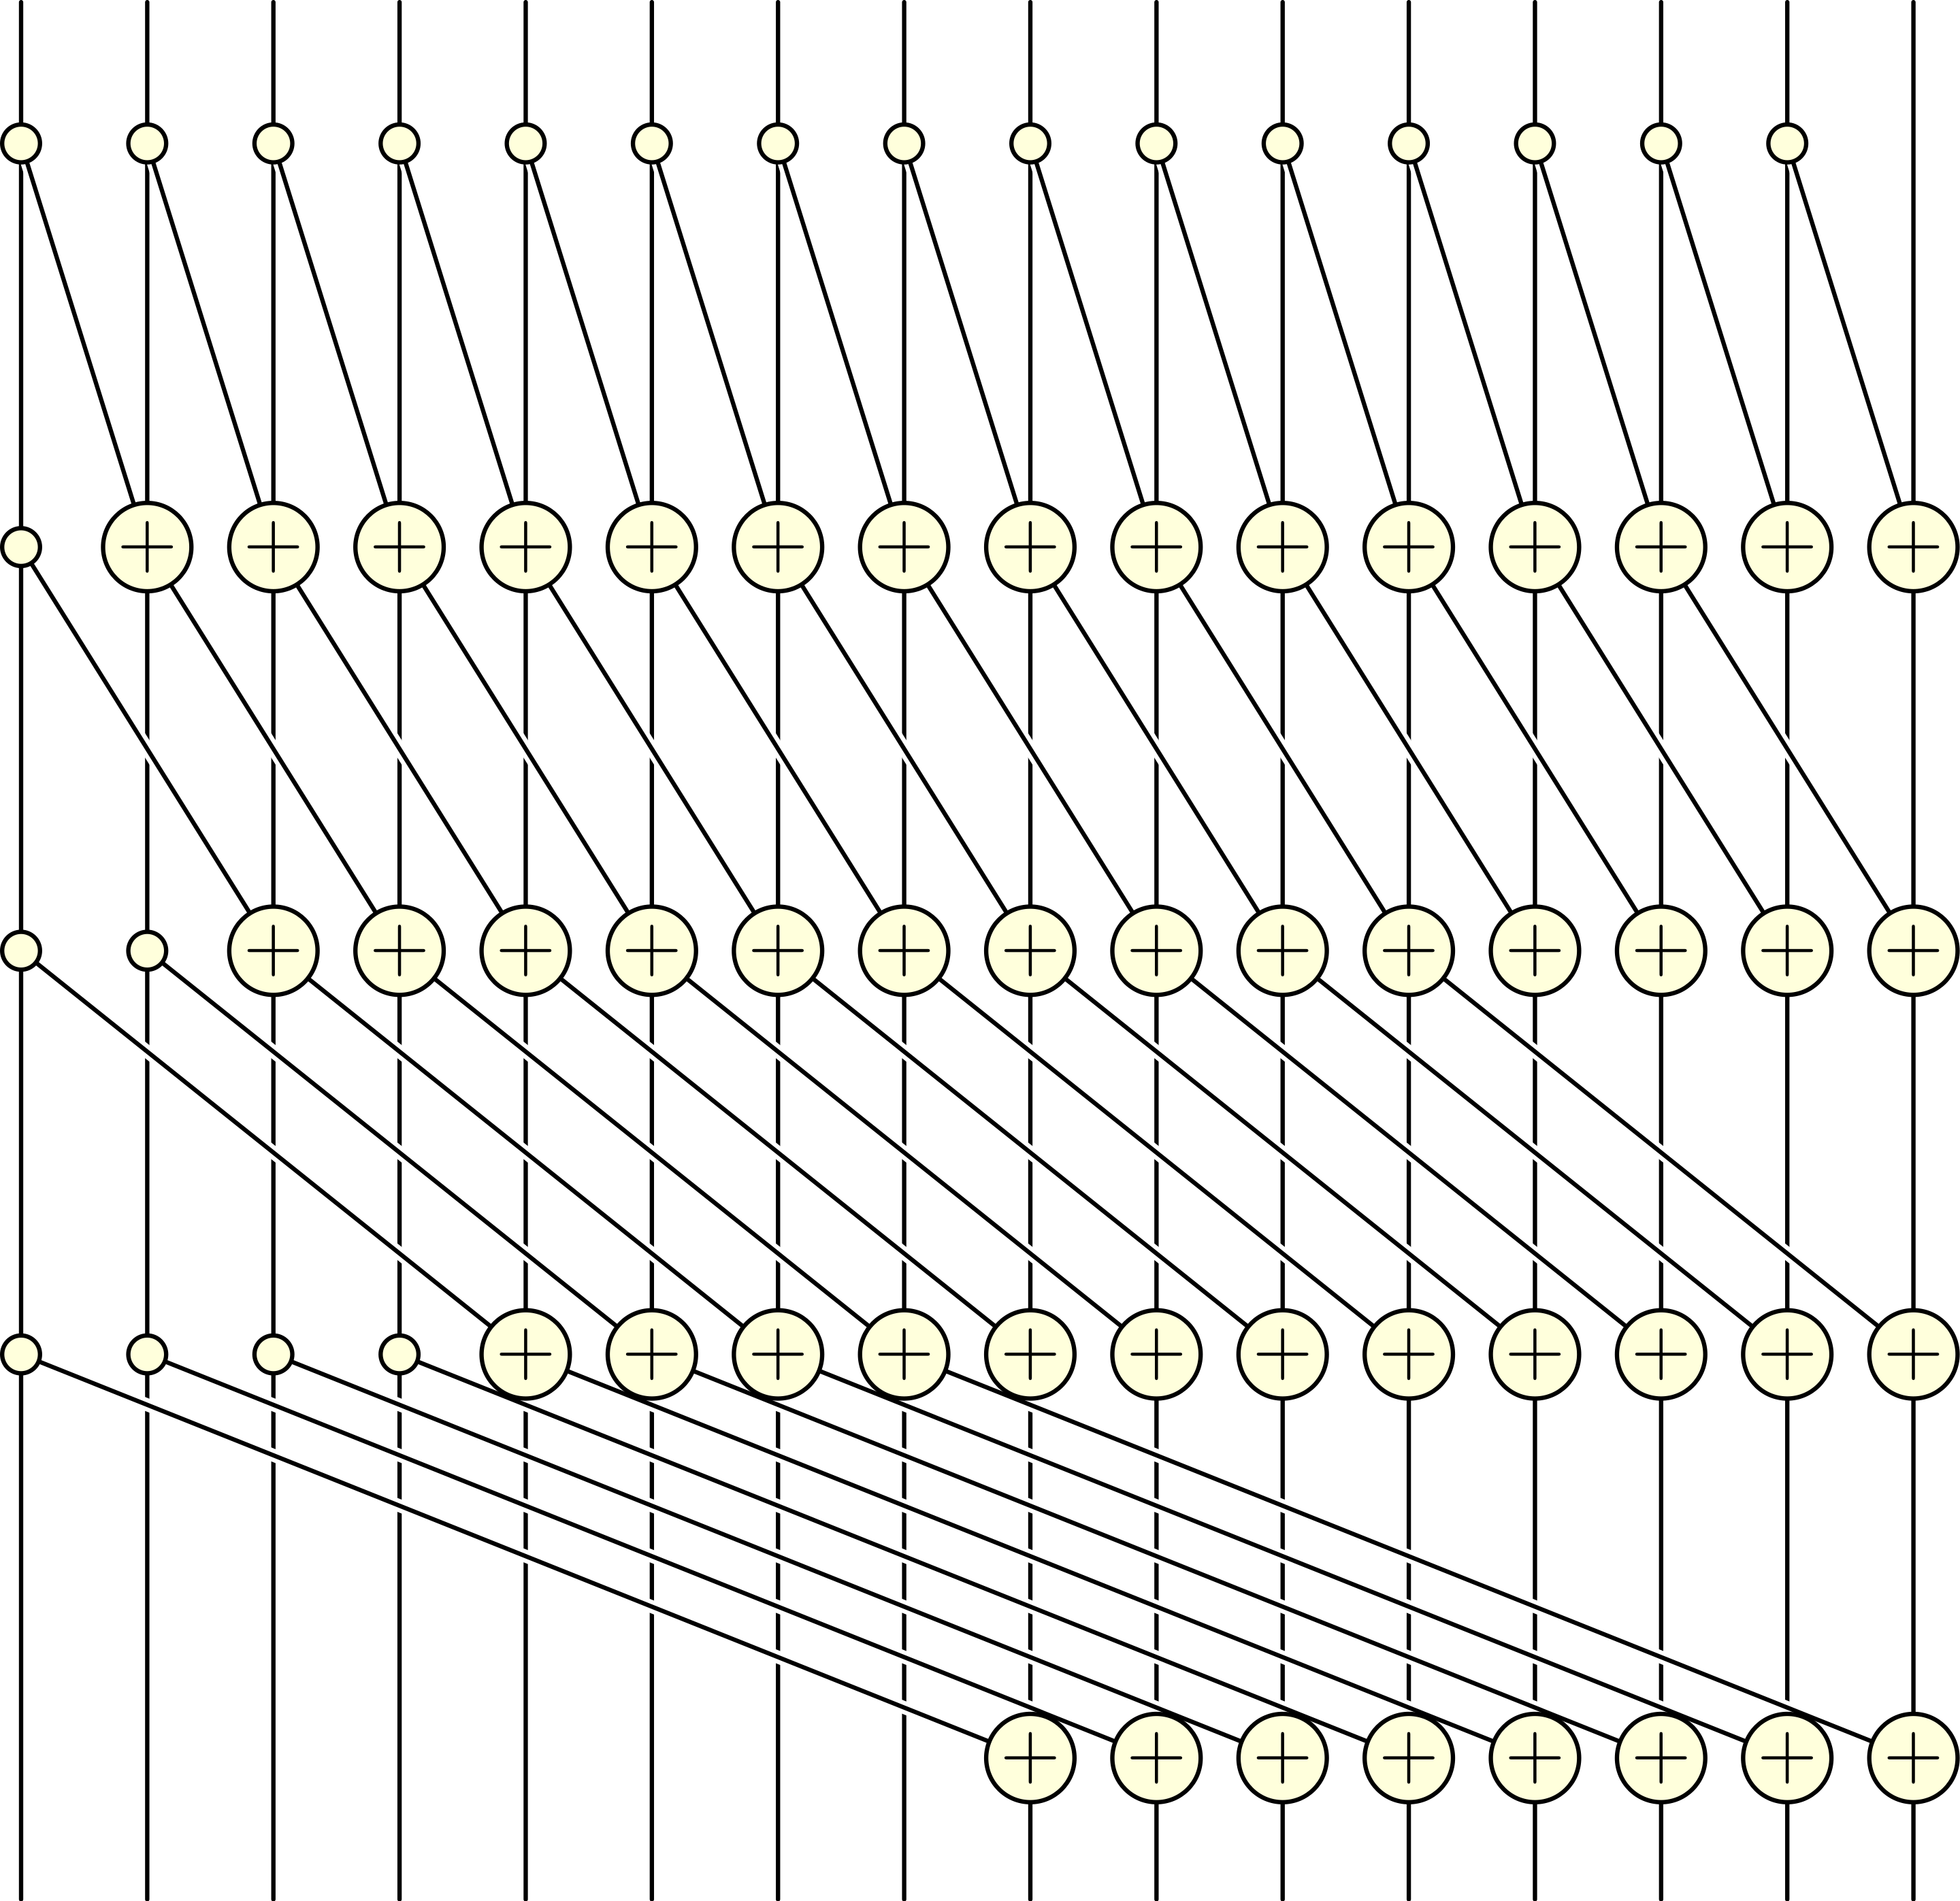
\includegraphics[width=0.8\textwidth]{Figuras/Hillis-Steele Prefix Sum.svg.png}
    \end{figure}
\end{frame}

\begin{frame}{Cenário experimental}
    Baterias de testes:
    \begin{itemize}
        \item[--] Algoritmos testados em diferentes arquiteturas.
        \item[--] 1 minuto de execução.
        \item[--] 3 execuções para aquecimento de \textit{cache}.
    \end{itemize} 
    \vspace{1em}
    Base de dados:
    \begin{itemize}
        \item[--] Mesma entrada para o mesmo algoritmo.
        \item[--] Carga de trabalho diferente para cada algoritmo.
        \item[--] Entradas geradas aleatoriamente.
    \end{itemize}
    \vspace{1em}
    Infraestrutura local do LabP2D:
    \begin{itemize}
        \item[--] 2 CPUs Intel Xeon Silver 2.2GHz.
        \item[--] NVIDIA RTX 3090 24GB.
    \end{itemize}
\end{frame}

\begin{frame}{Métricas de Avaliação}
    Estatísticas coletadas:
    \begin{itemize}
        \item[--] Média, Mediana, $R^2$, Desvio Padrão, \textit{MAD} e \textit{Slope}.
    \end{itemize}
    \vspace{1em}
    Métricas:
    \begin{itemize}
        \item[--] Speedup, Eficiência, Escalabilidade, Overhead.
    \end{itemize}
\end{frame}

\begin{frame}{Bateria de Testes}
    5 algoritmos testados.
    \begin{itemize}
        \item 5 Implementações seriais.
        \item 5 Implementações paralelas em CPU.
        \item 3 Implementações paralelas em GPU.
    \end{itemize}
    13 Implementações no total.
    \vspace{1em}
    \begin{itemize}
        \item 6 métricas coletadas.
        \item 11 gráficos por Implementação.
        \item 26 gráficos presentes no trabalho.
        \item Os demais estão presentes no \textit{GitHub}.
    \end{itemize}
\end{frame}

\begin{frame}{Gráfico de Densidade -- Prefix Sum CPU}
    \begin{figure}
        \centering
        \resizebox{\textwidth}{!}{
            \includesvg{Figuras/prefix-sum_cpu_pdf.svg}
        }
    \end{figure}
\end{frame}

\begin{frame}{Gráfico de Regressão -- Prefix Sum CPU}
    \begin{figure}
        \centering
        \resizebox{\textwidth}{!}{
            \includesvg{Figuras/prefix-sum_cpu_times.svg}
        }
    \end{figure}
\end{frame}

\begin{frame}{Resumo dos Tempos de Execução}
    \begin{table}[h!]
        \centering
        \resizebox{\linewidth}{!}{
        \begin{tabular}{|c|c|c|}
        \hline
        \textbf{Algoritmo} & \textbf{Arquitetura} & \textbf{Média de Tempo de Execução} \\
        \hline
        \textbf{Binary} & Serial & 503,32 ms \\
        \textbf{Search} & CPU & 24,66 ms \\
        \hline
        \textbf{Floyd} & Serial & 2,22 s \\
        \textbf{Warshall} & CPU & 692,05 ms \\
         & GPU & 24,77 ms \\
        \hline
        \textbf{Gaussian} & Serial & 2,55 s \\
        \textbf{Elimination} & CPU & 269,07 ms \\
         & GPU & 1,64 s \\
        \hline
        \textbf{Prefix} & Serial & 1,26 ms \\
        \textbf{Sum} & CPU & 421,35 µs \\
         & GPU & 63,93 ms \\
        \hline
        \textbf{Radix} & Serial & 3,50 s \\
        \textbf{Sort} & CPU & 1,65 s \\
        \hline
        \end{tabular}
        }
    \end{table}
\end{frame}

\begin{frame}{Resultados Speedup}
    \begin{table}[h!]
        \centering
        \resizebox{\linewidth}{!}{
        \begin{tabular}{|c|c|c|c|c|}
        \hline
        \textbf{Algoritmo} & \textbf{Arquitetura} & \textbf{Tempo} & \textbf{Tempo} & \textbf{Speedup} \\
        & & \textbf{Serial} & \textbf{Paralelo} & \\
        \hline
        \textbf{Binary Search} & CPU & 503,28 ms & 24,66 ms & 20,41 \\
        \hline
        \textbf{Floyd} & CPU & 2,22 s & 692,05 ms & 3,21 \\
        \textbf{Warshall} & GPU & 2,22 s & 24,77 ms & 89,64 \\
        \hline
        \textbf{Gaussian} & CPU & 2,55 s & 269,07 ms & 9,47 \\
        \textbf{Elimination} & GPU & 2,55 s & 1,64 s & 1,55 \\
        \hline
        \textbf{Prefix Sum} & CPU & 1,26 ms & 421,35 µs & 2,99 \\
         & GPU & 1,26 ms & 63,93 ms & 0,02 \\
        \hline
        \textbf{Radix Sort} & CPU & 3,50 s & 1,65 s & 2,12 \\
        \hline
        \end{tabular}
        }
    \end{table}
\end{frame}

\begin{frame}{Resultados Overhead}
    \begin{table}[h!]
        \centering
        \resizebox{\linewidth}{!}{
        \begin{tabular}{|c|c|c|c|c|}
        \hline
        & & \textbf{Tempo} & \textbf{Tempo} & \\
        \textbf{Algoritmo} & \textbf{Arquitetura} & \textbf{Paralelo} & \textbf{Paralelo} & \textbf{Overhead} \\
        & & \textbf{Ideal} & \textbf{Real} & \\
        \hline
        \textbf{Binary Search} & CPU & 10,48 ms & 24,66 ms & 14,18 ms \\
        \hline
        \textbf{Floyd} & CPU & 46,25 ms & 692,05 ms & 645,80 ms \\
        \textbf{Warshall} & GPU & 211,85 µs & 24,77 ms & 24,56 ms \\
        \hline
        \textbf{Gaussian} & CPU & 53,13 ms & 269,07 ms & 215,94 ms \\
        \textbf{Elimination} & GPU & 243,16 µs & 1,64 s & 1,64 s \\
        \hline
        \textbf{Prefix Sum} & CPU & 26,25 µs & 421,35 µs & 395,10 µs \\
         & GPU & 120,04 ns & 63,93 ms & 63,93 ms \\
        \hline
        \textbf{Radix Sort} & CPU & 72,92 ms & 1,65 s & 1,57 s \\
        \hline
        \end{tabular}
        }
    \end{table}
\end{frame}